\documentclass[prb,aps,twocolumn,showpacs,10pt]{revtex4-1}
\pdfoutput=1
\usepackage{dcolumn}% Align table columns on decimal point
\usepackage{bm}% bold math

%\usepackage{anysize}
\usepackage[colorlinks,hyperindex, urlcolor=blue, linkcolor=blue,citecolor=black, linkbordercolor={.7 .8 .8}]{hyperref}
\usepackage{graphicx}
%\usepackage{tabularx}
\usepackage{amsfonts}
\usepackage{amsmath}
\usepackage{amssymb}
\usepackage{amsbsy}
\usepackage{tikz}
\usepackage{caption}
\usepackage{subcaption}
\usepackage{nicefrac}
\usetikzlibrary{arrows,shapes,positioning}
\newenvironment{psmallmatrix}
  {\left[\begin{matrix}}
  {\end{matrix}\right]}
\usetikzlibrary{arrows,shapes,positioning}
\usetikzlibrary{decorations.markings}
  
 \usepackage{listings}
\usepackage{color}

\definecolor{dkgreen}{rgb}{0,0.6,0}
\definecolor{gray}{rgb}{0.5,0.5,0.5}
\definecolor{mauve}{rgb}{0.58,0,0.82}

\lstset{frame=tb,
  language=Java,
  aboveskip=3mm,
  belowskip=3mm,
  showstringspaces=false,
  columns=flexible,
  basicstyle={\small\ttfamily},
  numbers=none,
  numberstyle=\tiny\color{gray},
  keywordstyle=\color{blue},
  commentstyle=\color{dkgreen},
  stringstyle=\color{mauve},
  breaklines=true,
  breakatwhitespace=true,
  tabsize=3
}


\newcommand{\etal}{{\it et~al.}}

\graphicspath{{figures/}}

\begin{document}

\title {Project 3}

\author{Jane Kim}
\affiliation{Physics 480: Computational Physics}
\date{\today}


\begin{abstract}

\vspace*{5mm}
\noindent Summary, numbers.
\end{abstract}

\maketitle

\section{Introduction}
motivation, explain structure of report.

\section{Theory}

The physics background required for this project is not very extensive, as the only force involved is gravity. To start simply, consider two celestial bodies with masses $M_1$ and $M_2$ at the locations $(x_1,y_1)$ and $(x_2,y_2)$ on the $x$-$y$ plane. We can obtain two coupled differential equations for the motion of $M_2$
\begin{equation}
\begin{split}
\frac{d^2x_2}{dt^2} &= \frac{GM_1(x_1-x_2)}{((x_1-x_2)^2+(y_1-y_2)^2)^{3/2}}\\
\frac{d^2y_2}{dt^2} &= \frac{GM_1(y_1-y_2)}{((x_1-x_2)^2+(y_1-y_2)^2)^{3/2}}
\end{split}
\end{equation}
\noindent using Newton's second law. Now add more planets with masses $M_3, M_4, \ ..., M_n$ into the system. Then to find the equations of motion for the $j^{th}$ planet, we need to sum over the interactions between $M_j$ and all the other $M_k$'s:
\begin{equation}
\begin{split}
\frac{d^2x_j}{dt^2} &= \sum_{\substack{{k = 1}\\k \neq j}}^n \frac{GM_k(x_k-x_j)}{((x_k-x_j)^2+(y_k-y_j)^2)^{3/2}}\\
\frac{d^2y_j}{dt^2} &= \sum_{\substack{{k = 1}\\k \neq j}}^n \frac{GM_k(y_k-y_j)}{((x_k-x_j)^2+(y_k-y_j)^2)^{3/2}}
\end{split}
\end{equation}
\noindent This can easily be extended into three dimensions:
\begin{equation}
\begin{split}
&\frac{d^2x_j}{dt^2} = \sum_{\substack{{k = 1}\\k \neq j}}^n \frac{GM_k(x_k-x_j)}{r^3}\\
&\frac{d^2y_j}{dt^2} = \sum_{\substack{{k = 1}\\k \neq j}}^n \frac{GM_k(y_k-y_j)}{r^3}\\
&\frac{d^2z_j}{dt^2} = \sum_{\substack{{k = 1}\\k \neq j}}^n \frac{GM_k(z_k-z_j)}{r^3}\\
r = &\sqrt{(x_k-x_j)^2+(y_k-y_j)^2+(z_k-z_j)^2}
\end{split}
\end{equation}


using convenient units can simplify 

\section{Method}
\subsection{Forward Euler}
\subsection{Velocity Verlet}

\section{Implementation}


\section{Tests}

\section{Results}

\section{Conclusion}

\begin{figure*}
\centering
\begin{subfigure}{.5\textwidth}
  \centering
  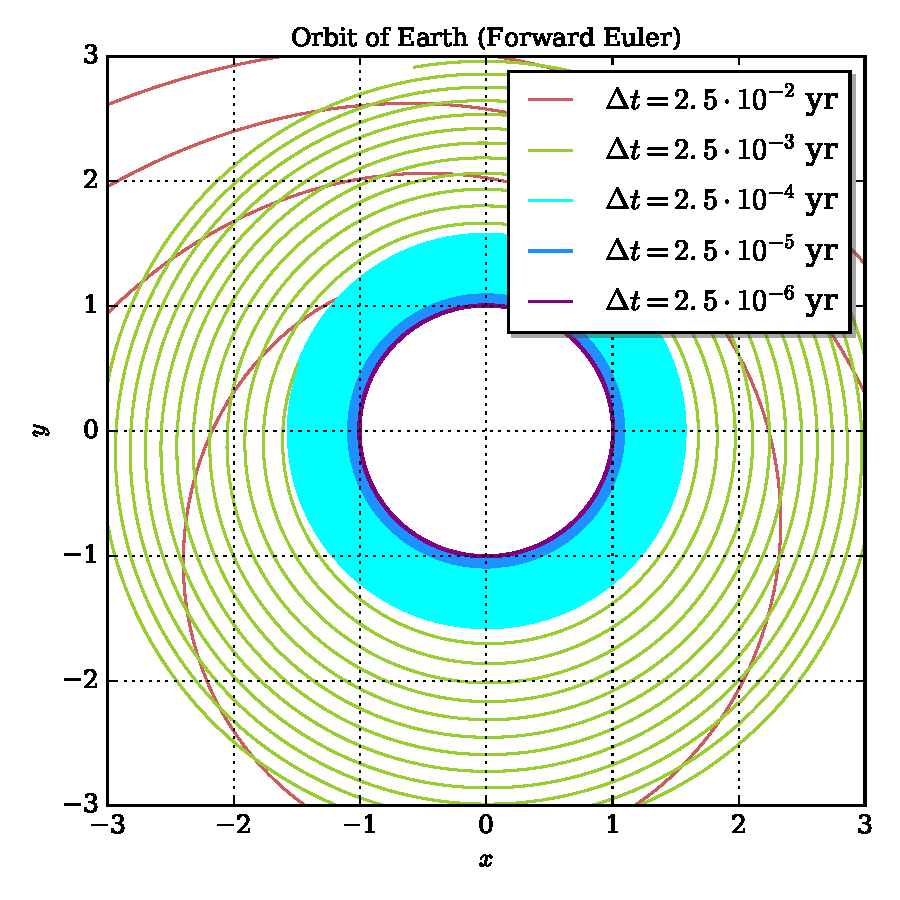
\includegraphics[width=\linewidth]{binary_fixed_euler_orbit.pdf}
  \caption{A subfigure}
  \label{fig:sub1}
\end{subfigure}%
\begin{subfigure}{.5\textwidth}
  \centering
  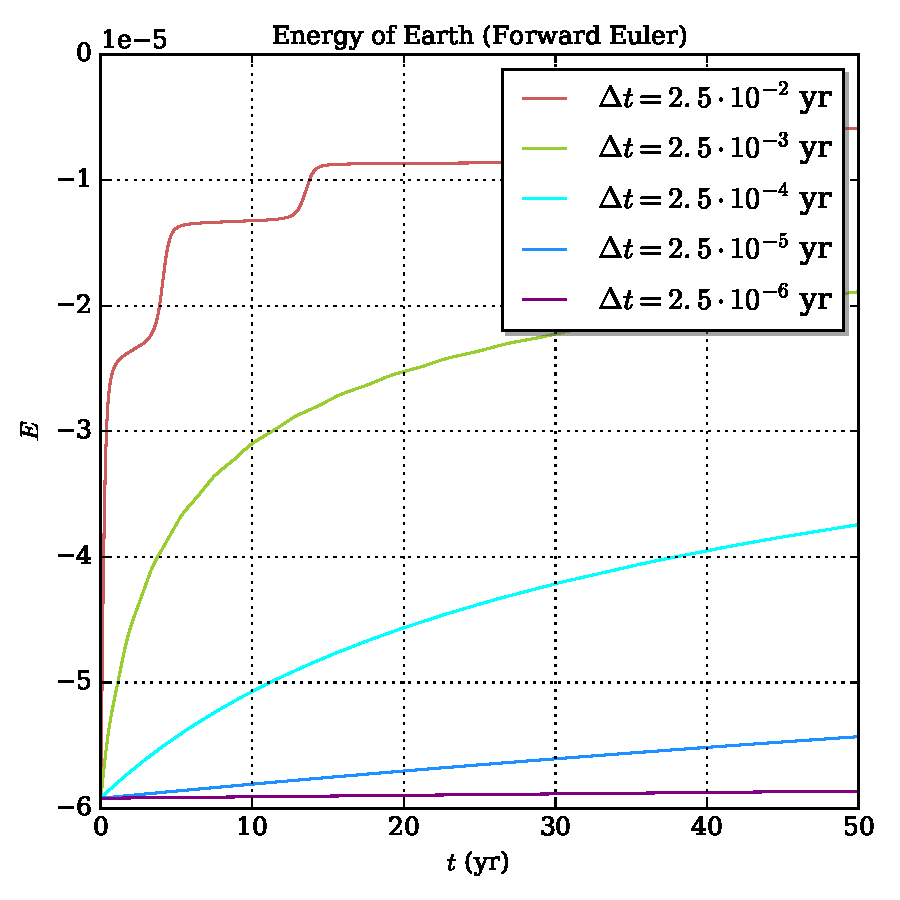
\includegraphics[width=\linewidth]{binary_fixed_euler_energy.pdf}
  \caption{A subfigure}
  \label{fig:sub2}
\end{subfigure}
\caption{A figure with two subfigures}
\label{fig:test}
\end{figure*}
\newpage
\begin{figure*}
\centering
\begin{subfigure}{.5\textwidth}
  \centering
  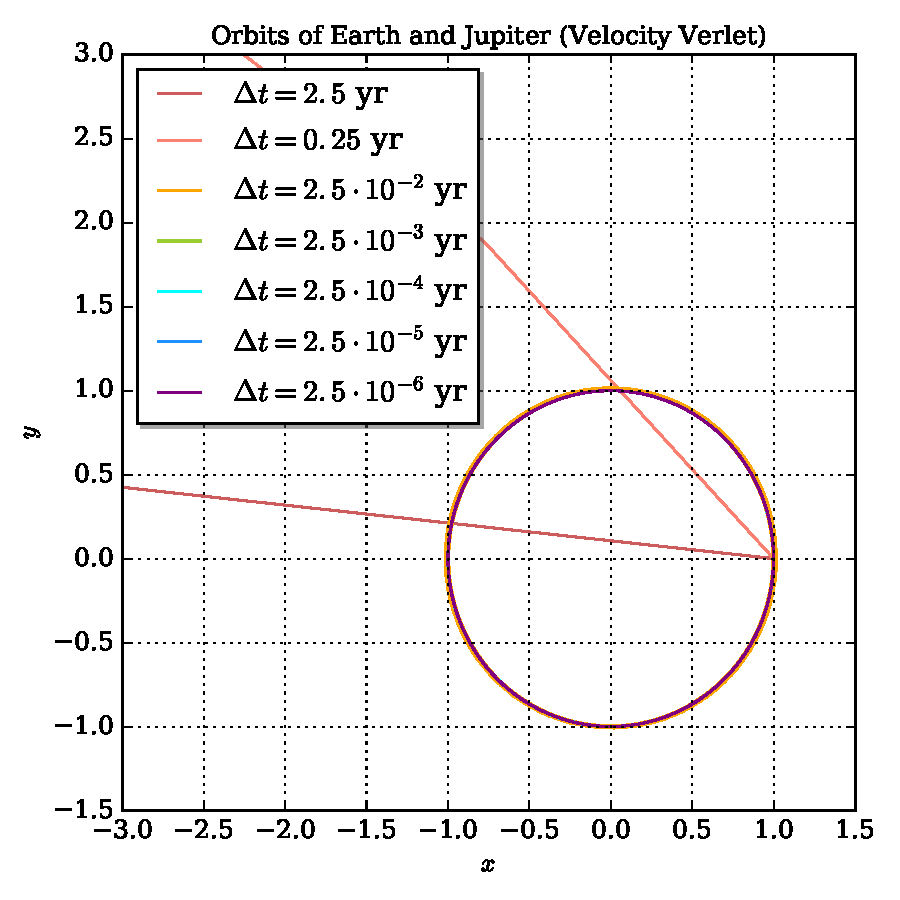
\includegraphics[width=\linewidth]{binary_fixed_vv_orbit.pdf}
  \caption{A subfigure}
  \label{fig:sub1}
\end{subfigure}%
\begin{subfigure}{.5\textwidth}
  \centering
  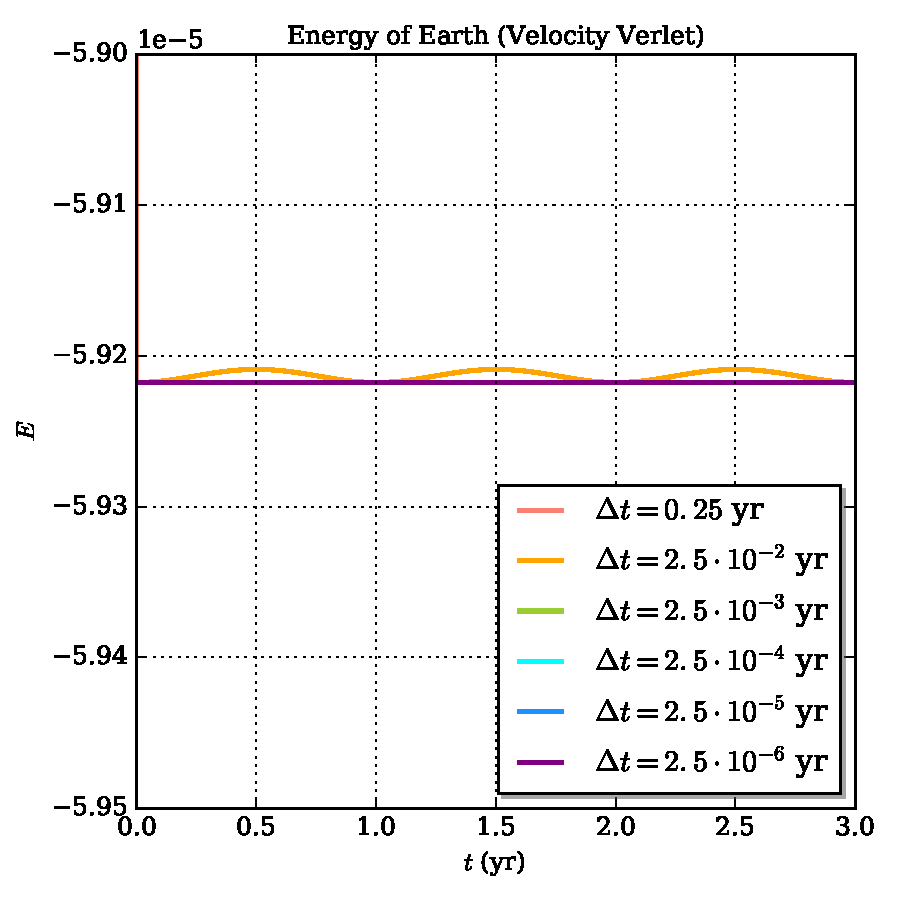
\includegraphics[width=\linewidth]{binary_fixed_vv_energy.pdf}
  \caption{A subfigure}
  \label{fig:sub2}
\end{subfigure}
\caption{A figure with two subfigures}
\label{fig:test}
\end{figure*}

\begin{figure}
\centering
\begin{subfigure}{.5\textwidth}
  \centering
  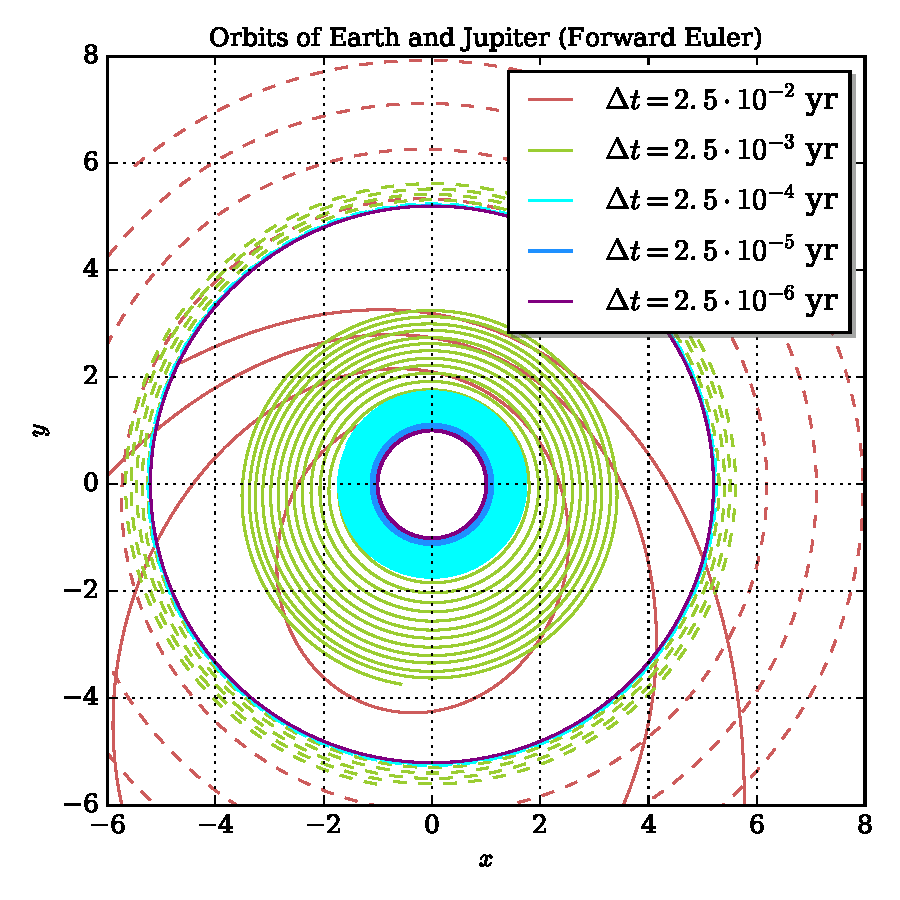
\includegraphics[width=\linewidth]{trinary_fixed_euler_orbit.pdf}
  \caption{A subfigure}
  \label{fig:sub1}
\end{subfigure}%
\begin{subfigure}{.5\textwidth}
  \centering
  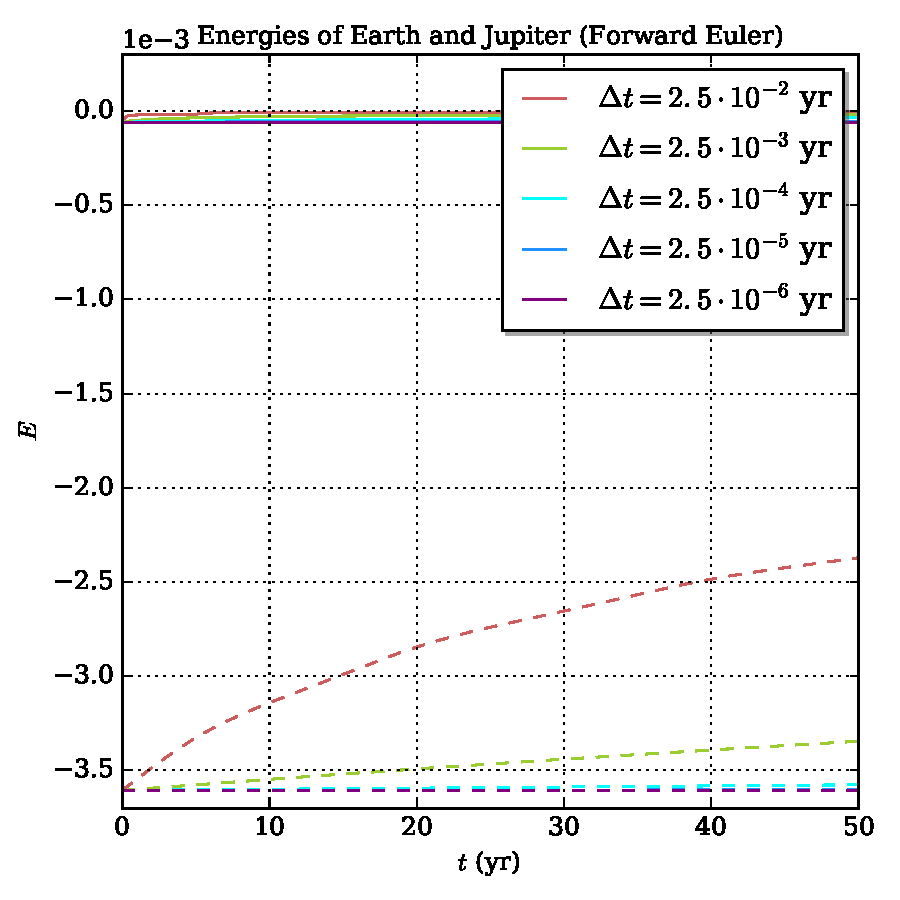
\includegraphics[width=\linewidth]{trinary_fixed_euler_energy.pdf}
  \caption{A subfigure}
  \label{fig:sub2}
\end{subfigure}
\caption{A figure with two subfigures}
\label{fig:test}
\end{figure}

\begin{figure}
\centering
\begin{subfigure}{.5\textwidth}
  \centering
  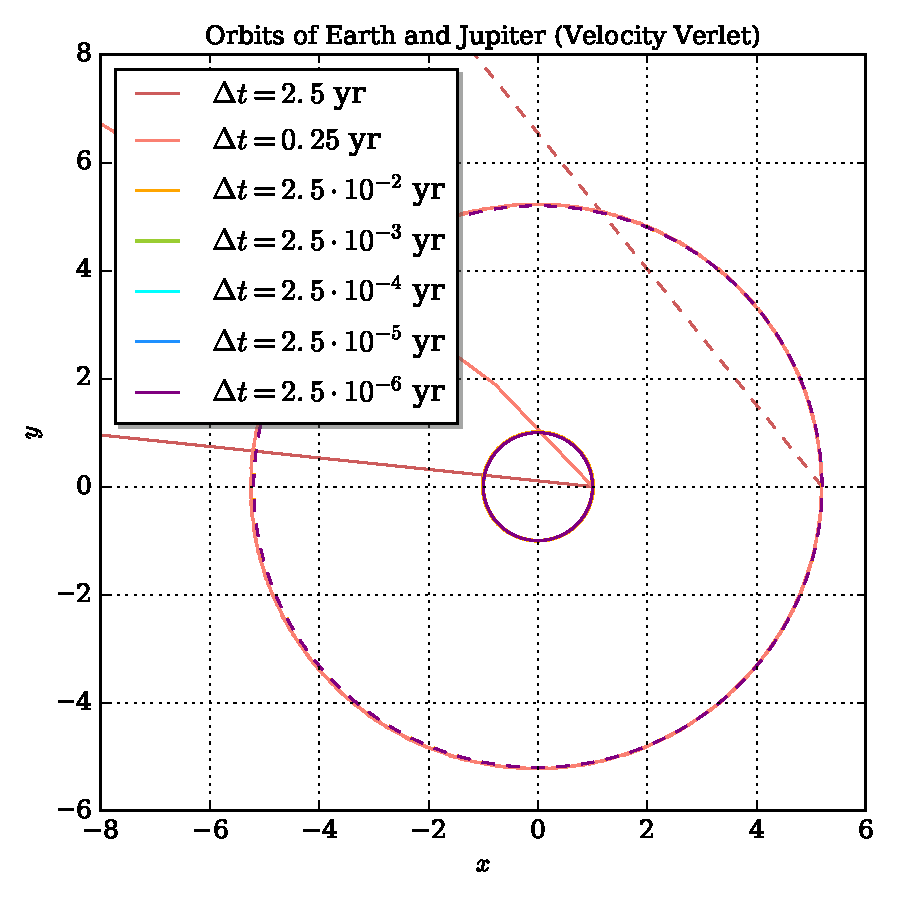
\includegraphics[width=\linewidth]{trinary_fixed_vv_orbit.pdf}
  \caption{A subfigure}
  \label{fig:sub1}
\end{subfigure}%
\begin{subfigure}{.5\textwidth}
  \centering
  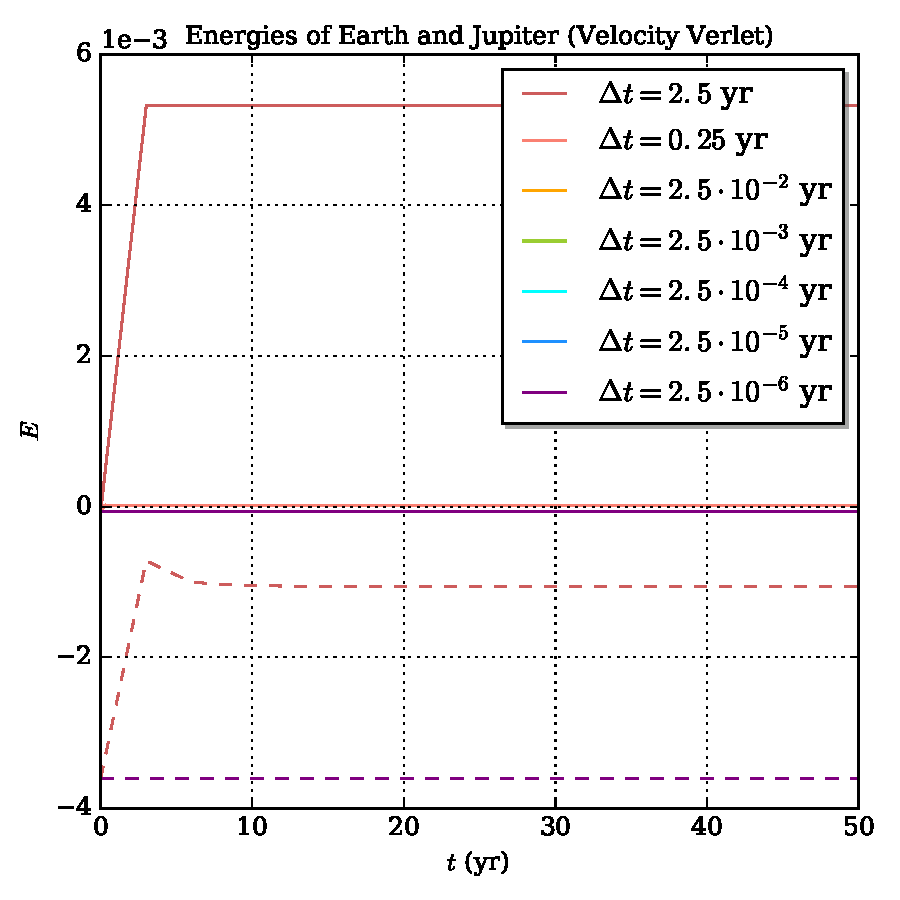
\includegraphics[width=\linewidth]{trinary_fixed_vv_energy.pdf}
  \caption{A subfigure}
  \label{fig:sub2}
\end{subfigure}
\caption{A figure with two subfigures}
\label{fig:test}
\end{figure}

\begin{figure}
\centering
\begin{subfigure}{.5\textwidth}
  \centering
  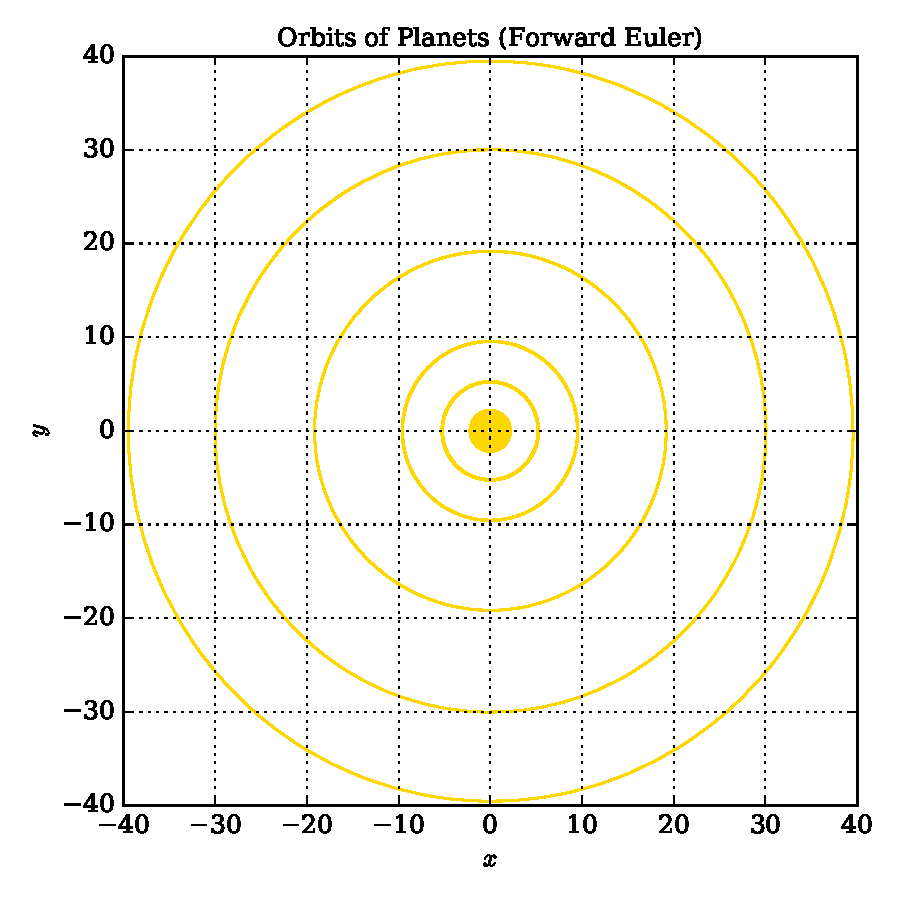
\includegraphics[width=\linewidth]{solar_system_euler_orbit.pdf}
  \caption{A subfigure}
  \label{fig:sub1}
\end{subfigure}%
\begin{subfigure}{.5\textwidth}
  \centering
  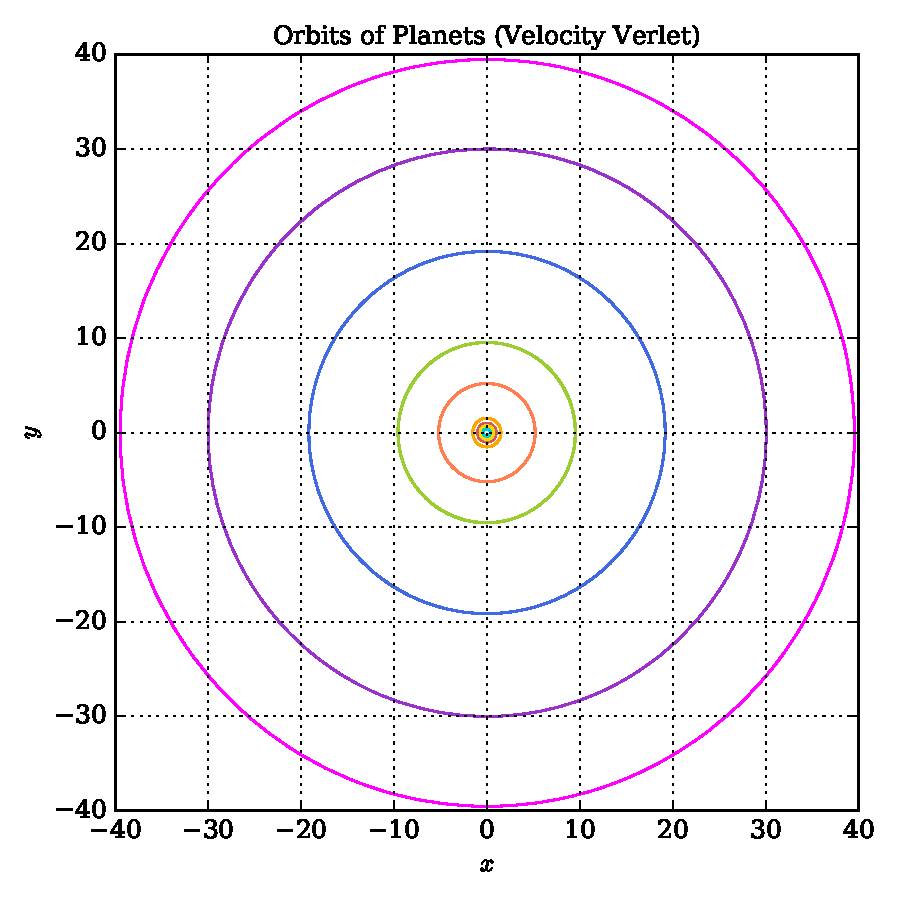
\includegraphics[width=\linewidth]{solar_system_vv_orbit.pdf}
  \caption{A subfigure}
  \label{fig:sub2}
\end{subfigure}
\caption{A figure with two subfigures}
\label{fig:test}
\end{figure}

\begin{center}
\begin{figure*}
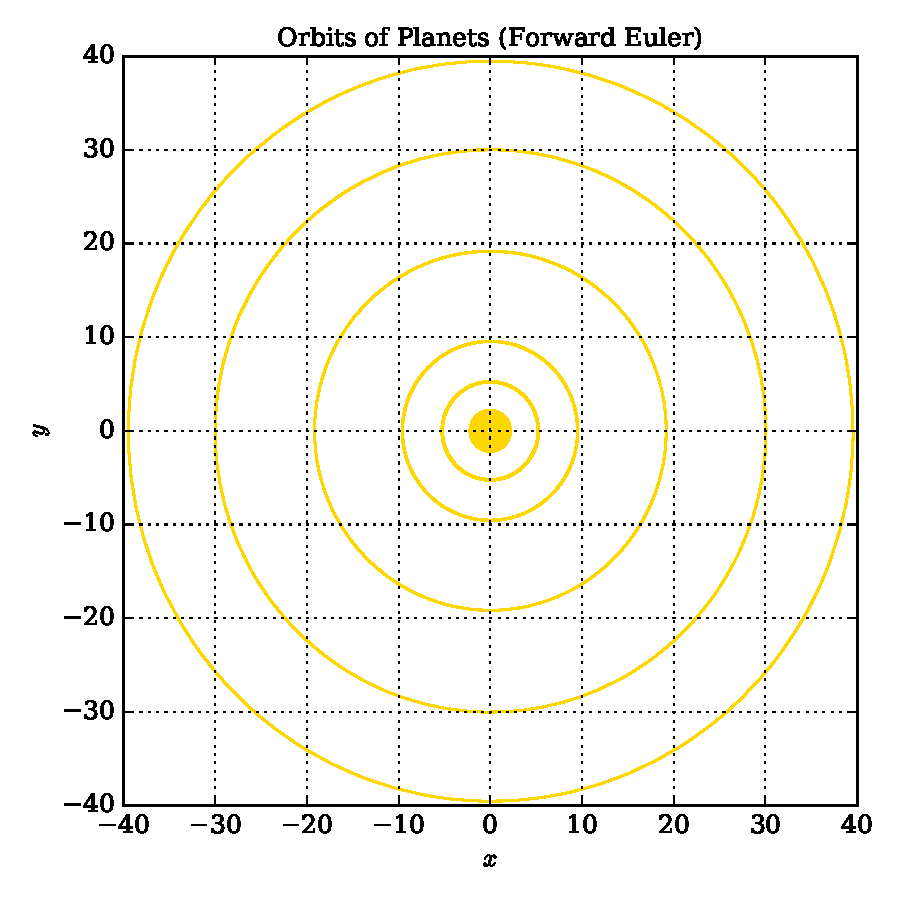
\includegraphics[scale=0.7]{solar_system_euler_orbit.pdf}
\end{figure*}
\end{center}
\begin{center}
\begin{figure*}
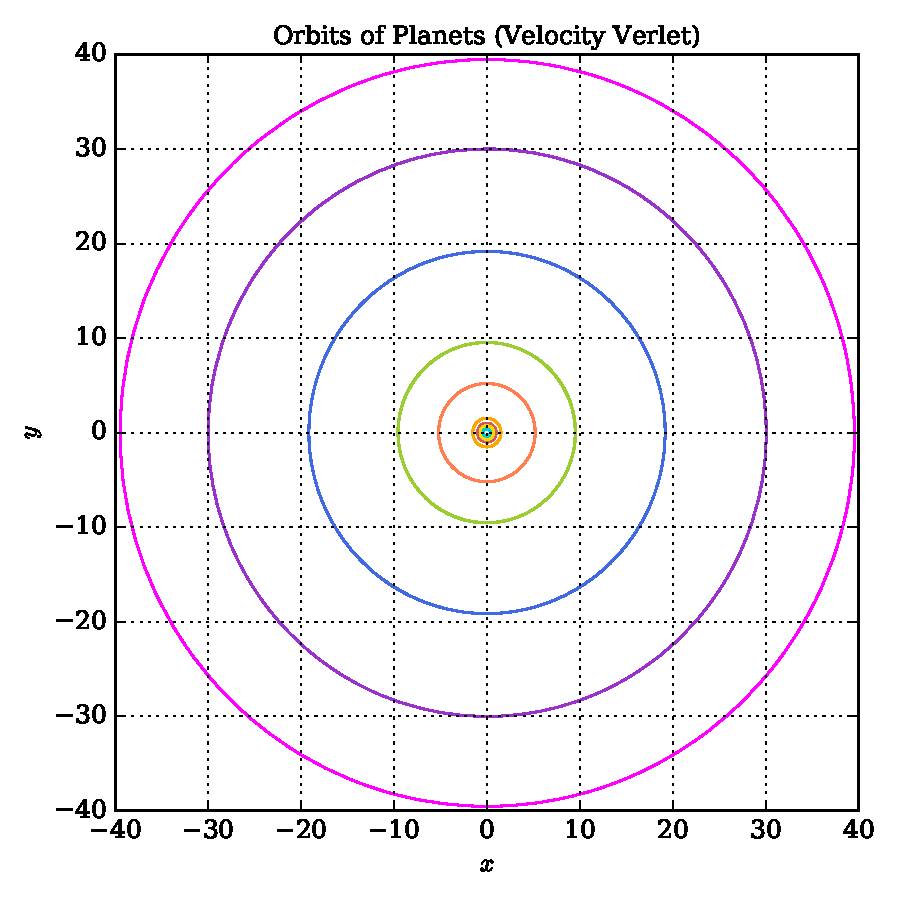
\includegraphics[scale=0.7]{solar_system_vv_orbit.pdf}
\end{figure*}
\end{center}


\newpage 
\begin{references}
\bibitem{notes} M. Hjorth-Jensen. "Computation Physics, Lecture Notes Fall 2015". University of Oslo. August 2015.
\end{references}

\end{document}
